\documentclass{standalone}

\usepackage{mintikz}
\usetikzlibrary{circuits.ee.IEC}
\usetikzlibrary{babel}

\begin{document}
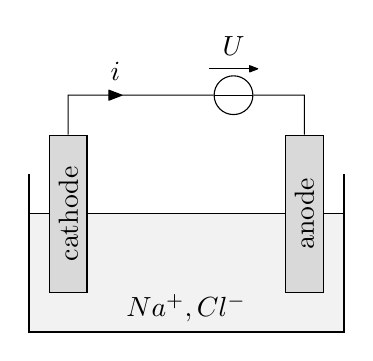
\begin{tikzpicture}[circuit ee IEC]
	%\usetikzlibrary{svg.path}%
	\fill [black!5] (-2, 1.5) rectangle (2, 0);
	\draw [thick] (-2, 2) |- (2, 0) -- (2, 2);
	\draw (-2, 1.5) -- (2, 1.5);
	\node at (0, 0) [above] {$\ce{Na^+, Cl^-}$};
	\node (cathode) at (-1.5, 1.5) [rotate=90, draw, fill=black!15, minimum width=20mm] {cathode};
	\node (anode) at (1.5, 1.5) [rotate=90, draw, fill=black!15, minimum width=20mm] {anode};
	\draw
	(cathode.east) -- ++(0, 0.5) coordinate (C)
	to [current direction={pos=0.2, info=$i$},
			voltage source={pos=0.7, direction info={info=$U$}}] (C -| anode.east) -- (anode.east);
\end{tikzpicture}%
\end{document}
